\scanpage{45}
\mspage{\handwritten{13}}
it suffices to see that if $\handwritten{\mathcal{F}}$ is flat over $\handwritten{\mathcal{O}}_S$, \inserted{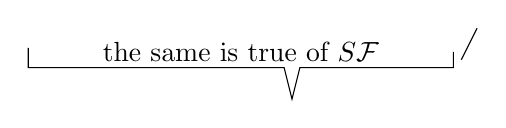
\begin{tikzpicture}[x=1cm,y=1cm,baseline=(n.base)]\node (n) at (0,0) {the same is true of $\handwritten{\mathbb{S}\mathcal{F}}$};\draw (-2.7,.05)--(-2.7,-.2)--(.55,-.2)--(.65,-.6)--(.75,-.2)--(2.7,-.2)--(2.7,0);\draw (2.8,-.1)--(3,.3);\end{tikzpicture}} which \deleted{follows from the definitions (EGA II 1.7.1), taking into account}\inserted{\handwritten{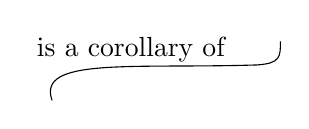
\begin{tikzpicture}[x=1cm,y=1cm,baseline=(n.base)]\node (n) at (0,0) {is a corollary of};\draw (-1,-.65) .. controls (-1.2,-.1) and (0,-.25) .. (1.6,-.2) .. controls (1.9,-.18) and (1.9,-.1) .. (1.9,.1);\end{tikzpicture}}} a result due to Daniel LAZARD, according to which every\deleted{ inductive limit of flat modules is a} flat module\deleted{.} \inserted{\handwritten{over a ring is a filtering inductive limit of free modules of finite type.}}

\deleted{Note moreover that $\handwritten{\unsure{\mathcal{A}|a}}(X)\handwritten{\otimes}_{\handwritten{\mathcal{O}}_S}\handwritten{\mathbb{S}\mathcal{F}}=\handwritten{\mathbb{S}}(\handwritten{\mathcal{A}}(X)\handwritten{\otimes}_{\handwritten{\mathcal{O}}_S}\handwritten{\mathcal{F}})$ by (EGA II 1.1.2), which shows that the canonical homomorphism $\handwritten{\mathcal{A}}(X)\handwritten{\otimes}_{\handwritten{\mathcal{O}}_S}\handwritten{\mathcal{F}\longrightarrow}\deleted{\handwritten{\mathbb{S}}}\handwritten{\mathcal{A}}(X)\handwritten{\otimes}_{\handwritten{\mathcal{O}}_S}\handwritten{\mathbb{S}\mathcal{F}}\deleted{\unsure{)}}$ is injective.}

Let us now show ii). Let $\handwritten{\alpha}$ be a morphism of $S$-functors from $X$ to $\handwritten{\mathcal{H}om}_{\handwritten{\mathcal{O}}_S}(\handwritten{\mathbb{V}}(\handwritten{\mathcal{F}}),\handwritten{\mathbb{V}}(\handwritten{\mathcal{E}}))$; to it corresponds a homomorphism $\handwritten{\rho}$ of $\handwritten{\mathcal{O}}_S$-Modules from $\handwritten{\mathcal{E}}$ to $\handwritten{\mathcal{A}}(X\handwritten{\times}_S\handwritten{\mathbb{V}}(\handwritten{\mathcal{F}}))=\handwritten{\mathcal{A}}(X)\handwritten{\otimes}_{\handwritten{\mathcal{O}}_S}\handwritten{\mathbb{S}}(\handwritten{\mathcal{F}})$ such that if $\handwritten{\rho}$ is an $S$-section of $X$, the homomorphism
\[
(\handwritten{\mathcal{A}(\eta)\otimes}\operatorname{id}_{\handwritten{\mathbb{S}\mathcal{F}}})\handwritten{\unsure{o|\circ}\rho}:\handwritten{\mathcal{E}\longrightarrow\mathcal{O}}_S\handwritten{\otimes}_{\handwritten{\mathcal{O}}_S}\handwritten{\mathbb{S}\mathcal{F}=\mathbb{S}\mathcal{F}}
\]
corresponds to $\handwritten{\alpha(\eta)}$. But since $\handwritten{\alpha(\eta)\in}\deleted{\handwritten{\unsure{\mathcal{E}|\mathcal{H}om}}}\handwritten{\mathcal{H}om}_{\handwritten{\mathcal{O}}_S}(\handwritten{\mathbb{V}}(\handwritten{\mathcal{F}}),\handwritten{\mathbb{V}}(\handwritten{\mathcal{E}}))(S)$, $\handwritten{\mathcal{A}(\eta)\otimes}\operatorname{id}_{\handwritten{\mathbb{S}\mathcal{F}}}$ factors through the canonical injective homomorphism $\handwritten{\mathcal{F}\to\mathbb{S}\mathcal{F}}$. We therefore have, for each $S$-section $\handwritten{\eta}$ of $X$\handwritten{,}a commutative diagram :
\margin{\handwritten{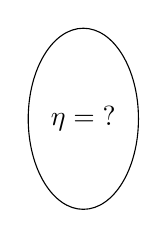
\begin{tikzpicture}
\draw (0,0) ellipse (.7 and 1.15);
\node at (0,0) {$\eta={?}$};
\end{tikzpicture}}}
\diagram{\handwritten{\begin{tikzcd}[ampersand replacement=\&]
\mathcal{E}\arrow[r,"\rho"]\arrow[d]\arrow[d,no head,shift left=1.2pt,shorten >=3pt] \& \mathcal{A}(X)\otimes\mathbb{S}\mathcal{F}\arrow[d]\arrow[dl,"\mathcal{A}(\eta)\otimes\operatorname{id}"']\\
\mathbb{S}\mathcal{F} \& \mathcal{F}\arrow[l]
\end{tikzcd}}}
\handwritten{,}

which shows that $\handwritten{\rho}$ factors through the canonical injective homomorphism $\handwritten{\mathcal{A}}(X)\handwritten{\otimes}_{\handwritten{\mathcal{O}}_S}\handwritten{\mathcal{F}\longrightarrow\mathcal{A}}(X)\handwritten{\otimes}_{\handwritten{\mathcal{O}}_S}\handwritten{\mathbb{S}\mathcal{F}}$ , hence $\handwritten{\rho}$ can be regarded as a homomorphism of $\handwritten{\mathcal{O}}_S$-Modules from $\handwritten{\mathcal{E}}$ to $\handwritten{\mathcal{A}}(X)\handwritten{\otimes}_{\handwritten{\mathcal{O}}_S}\handwritten{\mathcal{F}}$ .

Conversely, let $\handwritten{\rho\in}\operatorname{Hom}_{\handwritten{\mathcal{O}}_S\text{-}\mathrm{Mod.}}(\handwritten{\mathcal{E}}\ ,\ \handwritten{\mathcal{A}}(X)\handwritten{\otimes}_{\handwritten{\mathcal{O}}_S}\handwritten{\mathcal{F}})\handwritten{\subset}\operatorname{Hom}_{\handwritten{\mathcal{O}}_S\text{-}\mathrm{Mod}}(\handwritten{\mathcal{E}}\ ,\ \handwritten{\mathcal{A}}(X\handwritten{\times}_S\handwritten{\mathbb{V}}(\handwritten{\mathcal{F}})))$ ; to it corresponds a morphism $\handwritten{\alpha}$ from $X$ to $\handwritten{\mathcal{H}om}_{\unsure{\mathbb{S}|S}}(\handwritten{\mathbb{V}}(\handwritten{\mathcal{F}}),\handwritten{\mathbb{V}}(\handwritten{\mathcal{E}}))$ . For every $S$-prescheme $T$ and every $T$-section $\handwritten{\eta}$ of $X\handwritten{\times}_S T$ , $\handwritten{\alpha(\eta)}$ corresponds to $\handwritten{\mathcal{A}(\eta)\otimes}\operatorname{id}_{\handwritten{\mathbb{S}\mathcal{F}\otimes\mathcal{O}}_T}$ , a homomorphism from $\handwritten{\mathcal{E}\otimes}_{\handwritten{\mathcal{O}}_S}\handwritten{\mathcal{O}}_T$ to $\handwritten{\mathcal{F}\otimes}_{\handwritten{\mathcal{O}}_S}\handwritten{\mathcal{O}}_T$ , hence $\handwritten{d(\eta)\in\mathcal{H}om}_{\handwritten{\mathcal{O}}_S}(\handwritten{\mathbb{V}}(\handwritten{\mathcal{F}}),\handwritten{\mathbb{V}}(\handwritten{\mathcal{E}}))(T)$, which shows that $\handwritten{\alpha}$ is a morphism from $X$ to $\handwritten{\mathcal{H}om}_{\handwritten{\mathcal{O}}_S}(\handwritten{\mathbb{V}}(\handwritten{\mathcal{E}}),\handwritten{\mathbb{V}}(\handwritten{\mathcal{F}}))$, which proves ii).

\deleted{Corollary 11.6.- Let $G$ be an $S$-group flat, quasi-compact and quasi-separated over $S$, such that $\handwritten{\mathcal{A}}(G)$ is a flat $\handwritten{\mathcal{O}}_S$-module, \deleted{\unsure{and}} $\handwritten{\mathcal{E}}$ a quasi-coherent and flat $\handwritten{\mathcal{O}}_S$-Module. Then the set of linear maps}
% archive sheet number: 44
